\documentclass[11pt]{article}
\usepackage [french]{babel}
\usepackage [T1]{fontenc}

\usepackage[linesnumbered, ruled, french, onelanguage]{algorithm2e}
\usepackage{adjustbox}%Permet de centrer les figures dans la largeur de la page même si les figures sont plus larges que \textwidth
\usepackage{amssymb}
\usepackage{amsmath}
\usepackage{adjustbox} % pour avoir adjustbox
\usepackage[toc,page,title,titletoc,header]{appendix}
\usepackage{expl3}%Pour la control sequence /ExlpSyntaxOn demandée par l'utilisation de subfiles apparemment...
\usepackage{gensymb}%pour pouvoir écrire le signe °
%\usepackage{geometry}%Pour changer la largeur des marges du document notamment
\usepackage[paper=a4paper,margin=1in]{geometry}% http://ctan.org/pkg/geometry
\usepackage{graphicx}
\usepackage{hyperref}%pour les liens dans la bibliographie
\usepackage{listings}
\usepackage{placeins}%pour utiliser FloatBarrier afin que les figure respectent bien leur position dans le code
\usepackage{slashbox}%Case séparée en deux tout en haut à gauche des tableaux à double entrées
\usepackage{stmaryrd}%pour les crochets à double barres d'intervalles de nombre entiers
\usepackage{tikz}
\usepackage{xcolor}%/definecolor et /color
\usepackage{subfiles}
\usepackage[useregional]{datetime2}

\usepackage{etoolbox}%pour /AtBeginEnvironment
\AtBeginEnvironment{appendices}{\renewcommand{\thesection}{\Alph {section}}}%Pour recommencer à compter les sections à 0 en rentrant dans l'annexe et pour compter avec des lettres et non des chiffres
\renewcommand{\appendixpagename}{\centering Annexes}%Pour centrer le titre de la partie annexe
\renewcommand{\appendixtocname}{Table des annexes} % Pour faire apparaître les annexes dans la table of contents
\setlength{\parskip}{2mm}%Pour mettre de l'espacement entre les paragraphes

%TODO
% Images qui montrent les différences de résultats pour les différentes tailles de patch size : pour la brique, le pain et le panier

\author{Tom CLABAULT - p2205453\\}
\title{
\noindent\rule{\textwidth}{1pt}
\textit{\textbf{TP Bezier - Revolution - Deformations}}\\
\noindent\rule{\textwidth}{1pt}
%\vskip 1cm
}
\geometry{hmargin=1cm, vmargin=1cm}

\begin{document}

\maketitle
%\newgeometry{top=1in,bottom=1in,right=0.5in,left=1.5in}

\section{Courbes et surfaces de Bezier, déformations}
        	Les courbes et surfaces de Bézier ont été implémentées au moyen de 2 classes en C++. L'implémentation fait s'appuyer les surfaces de Bézier sur un ensemble de courbes de contrôle
qui elles même s'appuient sur un ensemble de points de contrôle.

La déformation globale de torsion agit sur tous les sommets du maillage et prend en paramètre un axe de torsion ainsi qu'une "intensité" de torsion exprimée en "degrés par unité" dans
les figures ci-dessous. Les 3 déformations locales (translations) appliquées à la surface de Bézier agissent sur tous les sommets du maillage mais l'intensité de la déformation
est modulée par une fonction à support compact de type smoothstep ($x^2(3 -2x)$) qui prend en argument la distance au centre de la déformation. Le centre de la déformation
est précisé par un des sommets du maillage dans cette implémentation.

\begin{figure}[h!]
	\adjustbox{center}{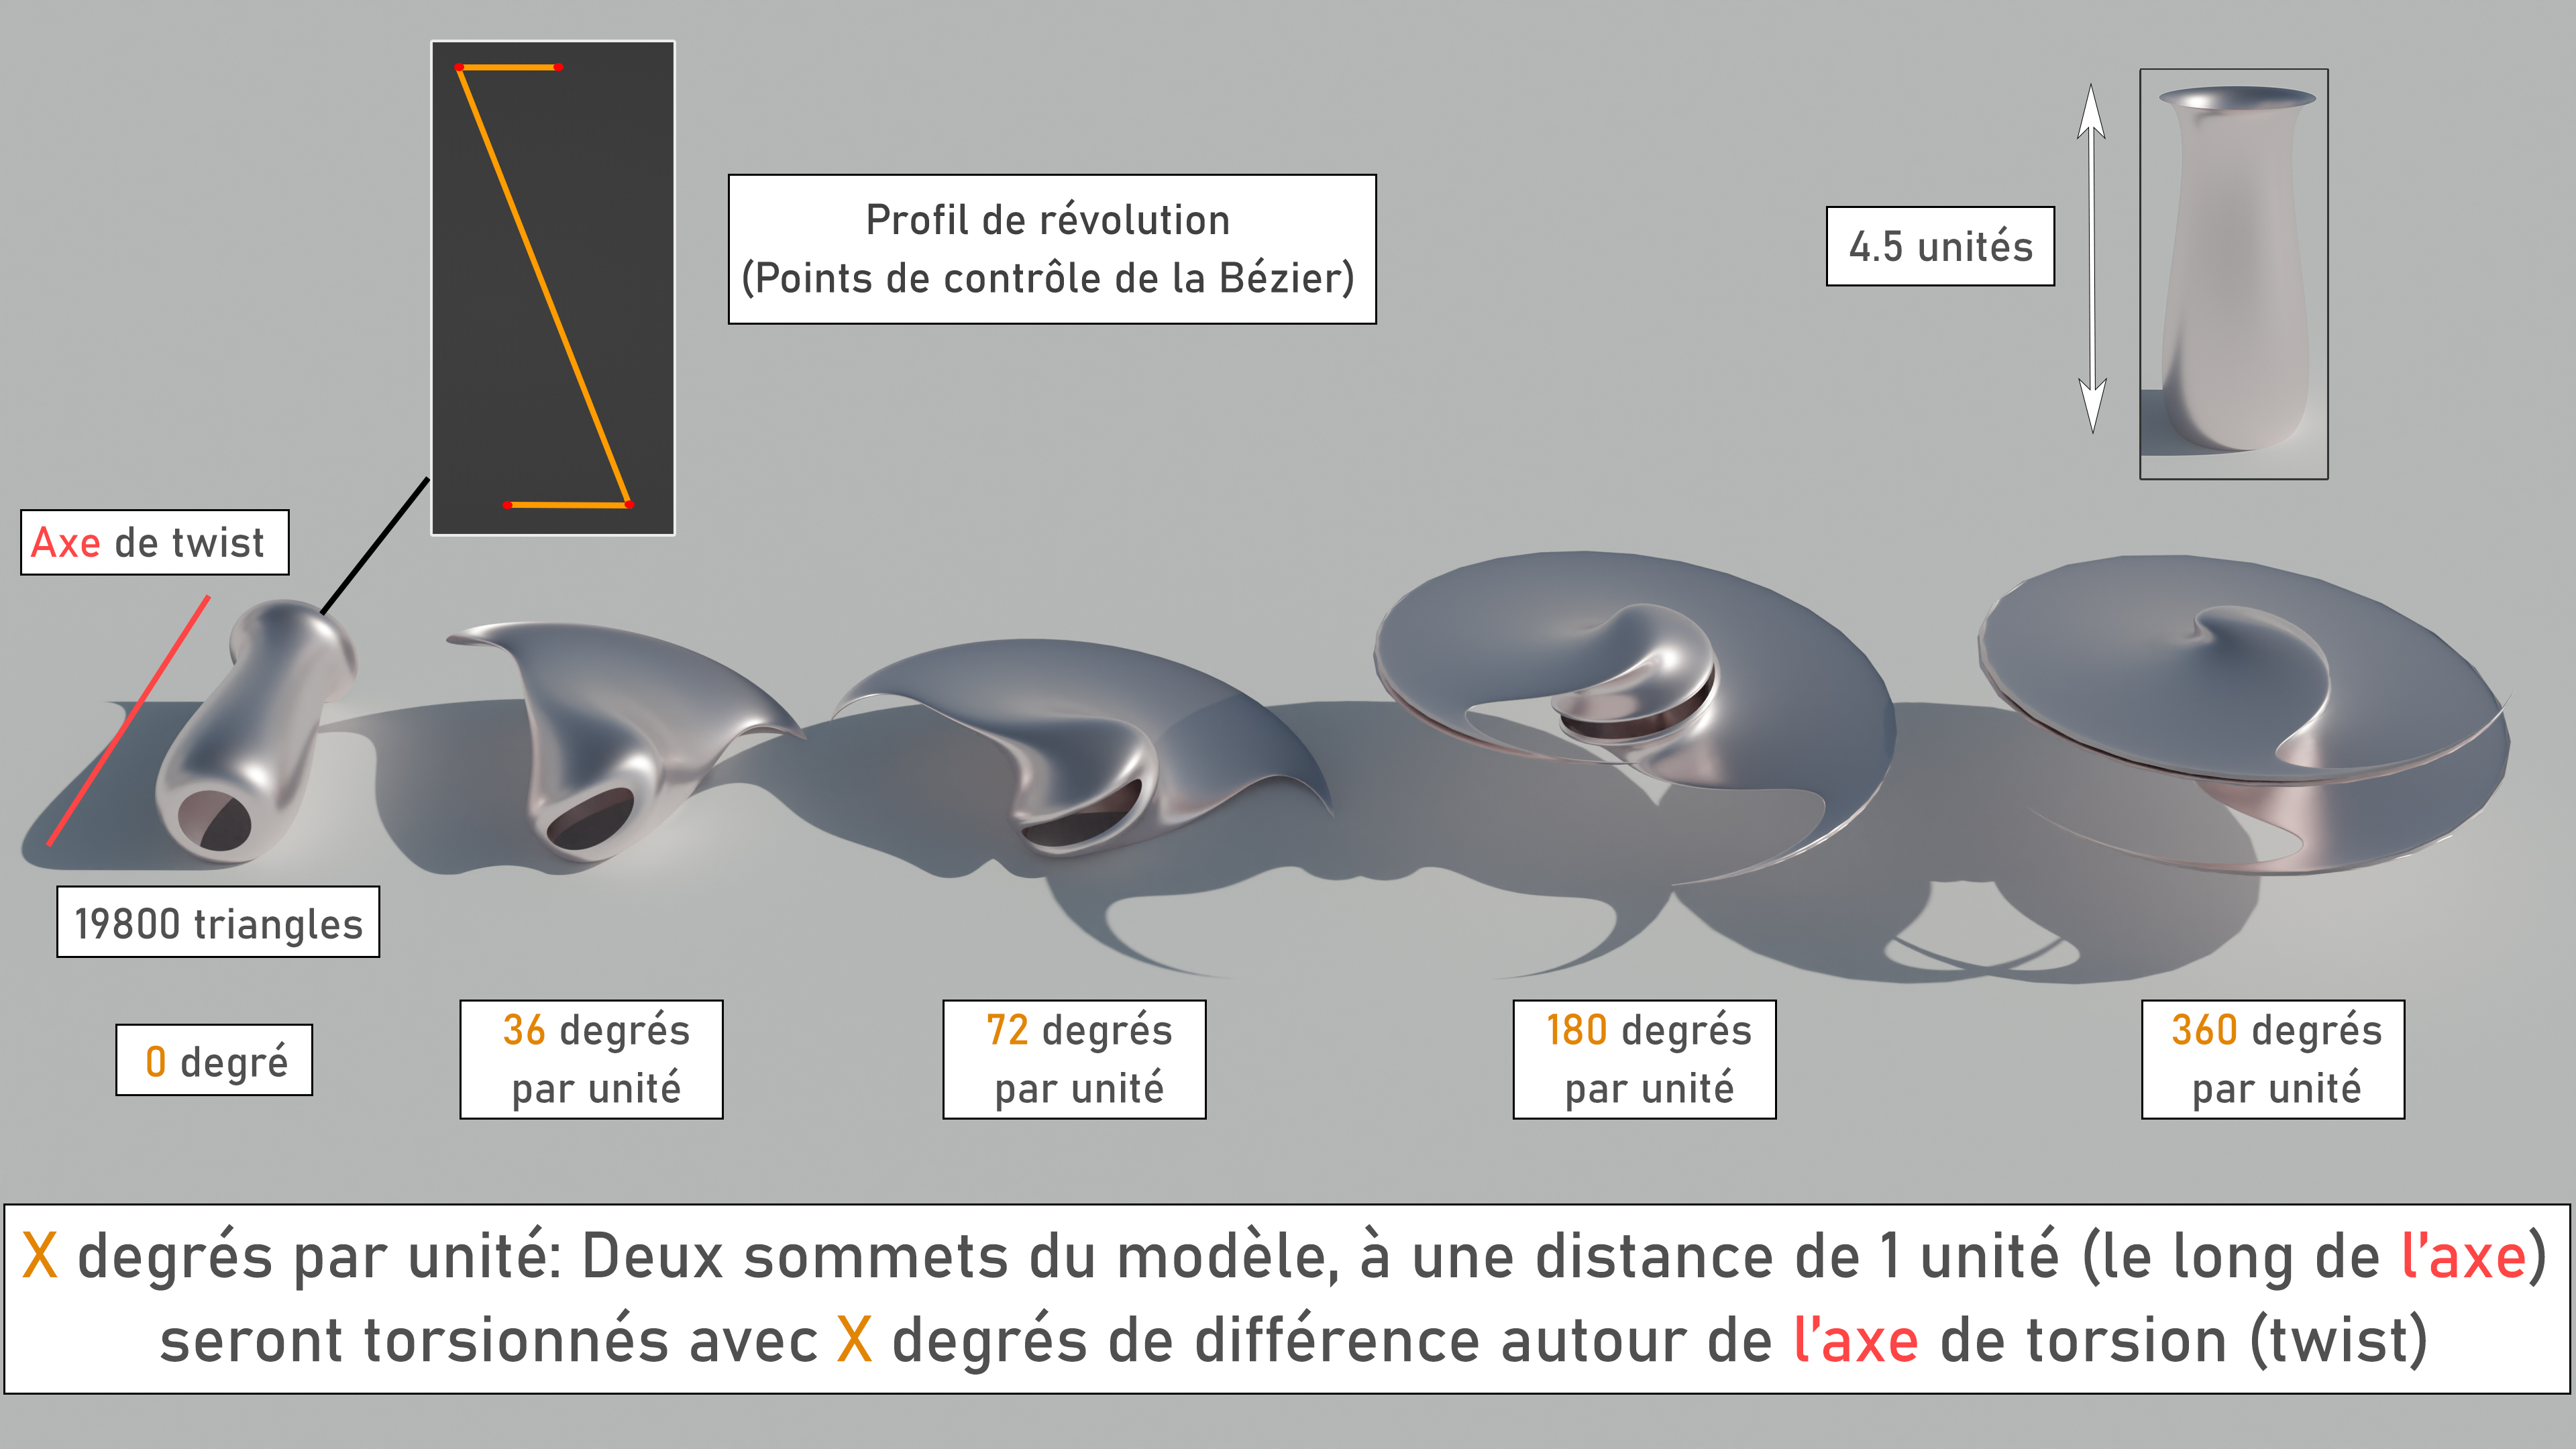
\includegraphics[width=1\textwidth]{Captures/Revolution.jpg}}

	\caption{Rendu Blender d'une surface de révolution modélisée, maillée et déformée globalement (torsion/twist) avec TinyMesh}
	\label{ref}
\end{figure}
\FloatBarrier

\begin{figure}[h!]
	\adjustbox{center}{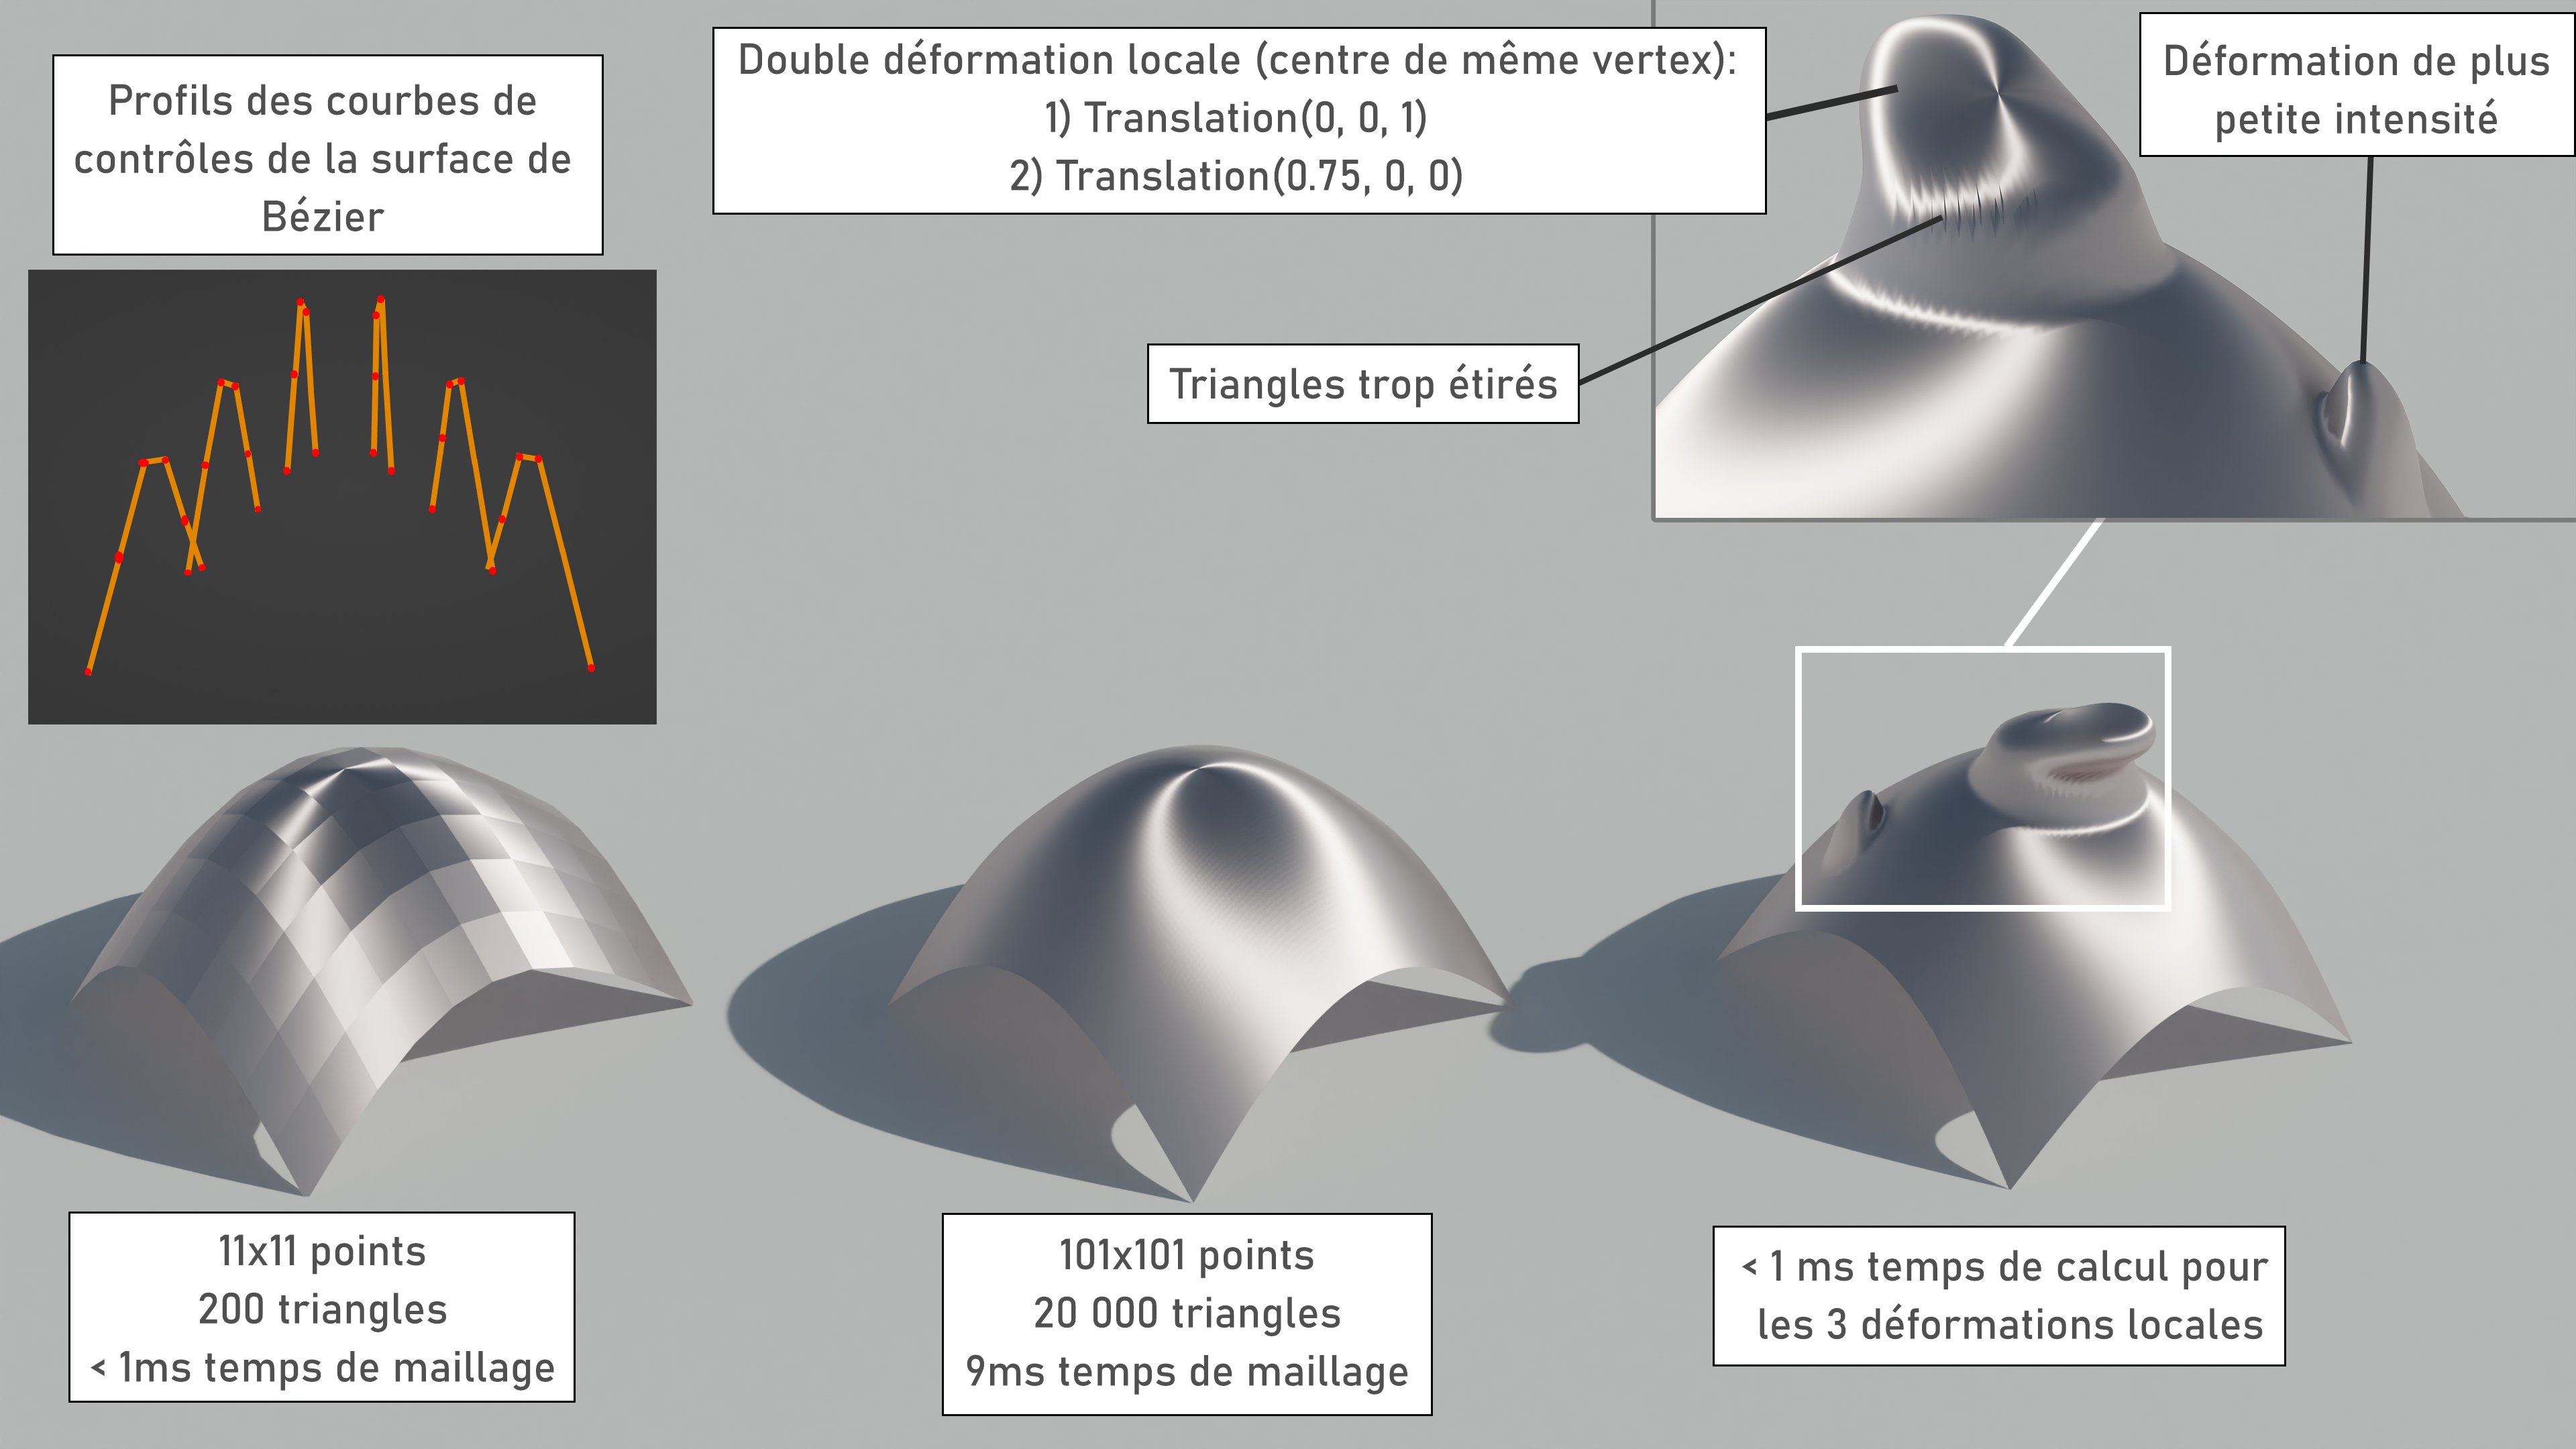
\includegraphics[width=1\textwidth]{Captures/Bezier.jpg}}

	\caption{Rendu Blender d'une surface de Bézier à différentes résolutions de maillage modélisée, maillée et déformée localement (translation atténuée) avec TinyMesh}
	\label{ref}
\end{figure}
\FloatBarrier

.



\end{document}
